\chapter{LPE structure}

\section{Introduction}
The LPE operations that are described in this document (see \ref{lpeoperations}) require a \txs{} model as input of which the process is in \emph{linear process equation} (LPE) \emph{form}.
Many, but not all \txs{} processes can be transformed to LPE form using the \texttt{lpe} command of \txs{}.

\section{LPE form} \label{lpeform}

A \txs{} process
\begin{align*}
\texttt{ProcDef} \; [C_1 :: K_1, \cdots{}, C_n :: K_n] \; [p_1 :: T_1, \cdots{}, p_k :: T_k] \; b_\textit{LPE}
\end{align*}

that is identified by $P$ is said to be a in \emph{LPE form} if $b_\textit{LPE}$ follows the grammar of $\textit{LPEBody}$ below:
\begin{align*}
\textit{LPEBody} &::= \texttt{Choice} \; [ \;\! \textit{ActionSmd}, \cdots{}, \textit{ActionSmd} \; ] \\
\textit{ActionSmd} &::= \texttt{ActionPref} \; \textit{ActOffer} \; \textit{ProcInst} \\
\textit{ActOffer} &::= \texttt{ActOffer} \; \textit{ChanOffers} \;\; [ \; h_1, \cdots{}, h_z \; ] \; \textit{VExpr} \\
\textit{ChanOffers} &::= [ \;\! \textit{ChanOffer}, \cdots{}, \textit{ChanOffer} \; ] \\
\textit{ChanOffer} &::= \textit{ChanId} \;\; [\texttt{Quest} \; x_1, \cdots{}, \texttt{Quest} \; x_m] \\
\textit{ChanId} &::= C_1 \;| \cdots{} |\; C_n \;|\; \texttt{ISTEP} \;|\; \texttt{CISTEP} \\
\textit{ProcInst} &::= \texttt{ProcInst} \; P \; \; [ \; C_1, \cdots{}, C_n \; ] \; [\;\!\textit{VExpr}, \cdots{}, \textit{VExpr} \; ]
\end{align*}

Note that
\begin{itemize}
\item $b_\textit{LPE}$ should comply with traditional \txs{} requirements.
More precisely, the communication variables $\{ x_1, \cdots{}, x_m \}$ must match the signature of the \textit{ChanId} channel that occurs in the same rule; and the number of \textit{VExpr}s in the \textit{ProcInst} rule must be equal to $k$ and their sorts must match $[T_1, \cdots{}, T_k]$.
\item it must be the case that the channels that are used in an \textit{ActionSmd} are either all input channels or all output channels.
\item per \textit{ActionSmd}, it must be the case that
\begin{align*}
|\; \{ h_1, \cdots{}, h_z \} \cup \{ x_1, \cdots{}, x_m \} \; | &= z + m \\
(\{ h_1, \cdots{}, h_z \} \cup \{ x_1, \cdots{}, x_m \}) \cap \{ p_1, \cdots{}, p_k \} &= \emptyset{}
\end{align*}
\end{itemize}

\section{Restricted LPE form} \label{restrictedlpeform}

In actuality, it is convenient that processes have a form that is even more restrictive than the LPE form discussed in \ref{lpeform}.
Fortunately, a process that is in LPE form can be converted to restricted LPE form in a way that is reversible.

The restricted LPE form is the same as the regular LPE form, except for the \textit{ActOffer} and \textit{ChanOffers} rules, which have changed to
\begin{align*}
\textit{ActOffer} &::= \texttt{ActOffer} \; \textit{ChanOffers} \;\; [\;] \; \textit{VExpr} \\
\textit{ChanOffers} &::= [ \;\! \textit{ChanOffer} \; ]
\end{align*}

In short, hidden variables are no longer permitted in the restricted LPE form, and there must be exactly one \textit{ChanOffer} per summand.

For the description of the conversion procedure, a more precise definition of the format of \txs{} models is used.
Let the form of a \txs{} model $M$ be
\begin{align*}
\texttt{ModelDef} \; [I_1, \cdots{}, I_m] \; [O_1, \cdots{}, O_n] \; b_\textit{inst}
\end{align*}

where

\begin{itemize}
\item $I_1, \cdots{}, I_m$ are all single input channels;
\item $O_1, \cdots{}, O_n$ are all single output channels;
\item $\{ I_1, \cdots{}, I_m \} \cap \{ O_1, \cdots{}, O_n \} = \emptyset{}$;
\item $b_\text{\textit{inst}}$ has the form
\begin{align*}
\texttt{ProcInst} \; P \; [D_1, \cdots{}, D_{m+n}] \; [v_I(p_1), \cdots{}, v_I(p_k)]
\end{align*}

such that
\begin{align*}
\{ D_1, \cdots{}, D_{m+n} \} = \{ I_1, \cdots{}, I_m \} \cup \{ O_1, \cdots{}, O_n \}
\end{align*}

\item the \txs{} process that is identified by $P$ is
\begin{align*}
\texttt{ProcDef} \; [C_1 :: K_1, \cdots{}, C_{m+n} :: K_{m+n}] \; [p_1 :: T_1, \cdots{}, p_k :: T_k] \; b_\textit{LPE}
\end{align*}
such that
\begin{align*}
\sortof{C_j} = \sortof{D_j} = K_j &\text{ for all } j \in [1, \cdots{}, m+n] \\
\sortof{v_I(p_j)} = T_j &\text{ for all } j \in [1, \cdots{}, k]
\end{align*}

and such that $b_\textit{LPE}$ follows the parametrized grammar of $\textit{LPEBody}$ below:
\begin{align*}
\textit{LPEBody} &::= \texttt{Choice} \; [ \;\! \textit{ActionSmd}(1), \cdots{}, \textit{ActionSmd}(s) \; ] \\
\textit{ActionSmd}(i) &::= \texttt{ActionPref} \; \textit{ActOffer}(i) \; \textit{ProcInst}(i) \\
\textit{ActOffer}(i) &::= \texttt{ActOffer} \; \textit{ChanOffers}(i) \; [ \; h_i(1), \cdots{}, h_i(z_i) \; ] \; g_i \\
\textit{ChanOffers}(i) &::= [ \;\! \textit{ChanOffer}_i(1), \cdots{}, \textit{ChanOffer}_i(m_i) \; ] \\
\textit{ChanOffer}_i(j) &::= c_i(j) \;\; [\texttt{Quest} \; x_{i,j}(1), \cdots{}, \texttt{Quest} \; x_{i,j}(|\flsortof{c_i(j)}|)] \\
\textit{ProcInst}_i(j) &::= \texttt{ProcInst} \; P \; \; [ \; C_1, \cdots{}, C_{m+n} \; ] \; [\;\!v_i(p_1), \cdots{}, v_i(p_k) \; ]
\end{align*}

where

\begin{itemize}
\item $s$ is the number of summands of $P$;
\item $h_i(j)$ is the $j$th hidden variable of the $i$th summand of $P$;
\item $z_i \geq 0$ is the number of hidden variables of the $i$th summand of $P$;
\item $g_i$ is the guard of the $i$th summand of $P$;
\item $m_i \geq 0$ is the number of channels over which the $i$th summand of $P$ communicates;
\item $c_i(j)$ is the $j$th channel over which the $i$th summand of $P$ communicates;
\item $\text{fl}(S_1 \; \texttt{\#\#} \cdots{} \texttt{\#\#} \; S_q) = [S_1, \cdots{}, S_q]$ for some $q > 0$;
\item $x_{i,j}(e)$ is the $e$th parameter that the $i$th summand of $P$ uses to communicate over channel $c_i(j)$;
\item $v_i(p)$ is an expression that defines the new value of parameter $p$ of $P$ after the application of summand $s_i$.
\end{itemize}
\end{itemize}

Furthermore, the conversion procedure will to refer to `channel signatures'.
A \emph{channel signature} is a pair $(C, S)$ where $C$ is an ordered list of channels and $S$ is an ordered list of sorts.
A function $\tau$ is defined that yields the channel signature of $s_i$, the $i$th summand of $P$:
\begin{align*}
\tau(s_i) = (&[ c_i(1), \cdots{}, c_i(m_i)], \\
&[\flsortof{c_i(1)}, \cdots{}, \flsortof{c_i(m_i)}, \sortof{h_i(1)}, \cdots{}, \sortof{h_i(z_i)}])
\end{align*}

Finally, define an injective function $\theta(T)$ that maps channel signatures of the form
\begin{align*}
T = (C, [S_1, \cdots{}, S_{m_i+z_i}])
\end{align*}

to a fresh, uniquely named channel with sort $S_1 \; \texttt{\#\#} \cdots{} \texttt{\#\#} \; S_{m_i+z_i}$.

Given the definitions above, do the following:

\begin{enumerate}
\item For each summand $s_i$, compute channel signature $\tau(s_i)$.
Add the result to a set $\Sigma_I$ if summand $s_i$ contains input actions, or add the result to a set $\Sigma_O$ if summand $s_i$ contains output actions (exactly one of these happens).

\item Compute $\Omega_I = \{ \; (\sigma, \theta(\sigma)) \;|\; \sigma \in \Sigma_I \; \}$ and $\Omega_O = \{ \; (\sigma, \theta(\sigma)) \;|\; \sigma \in \Sigma_O \; \}$.
Essentially, each channel signature is mapped to a fresh channel.

\item Compute the list $\Theta = [ \; \Theta_1, \cdots{}, \Theta_t \; ] = [ \; b \;|\; (a, b) \in \Omega_I \cup \Omega_O \; ]$.
The list $\Theta$ contains all fresh channels in some order.

\item For each summand $s_i$, look up a pair $(a, b) \in \Omega_I \cup \Omega_O$ so that $a = \tau(s_i)$.
By design, there is exactly one such pair.
Change the form of $s_i$ to
\begin{align*}
\textit{ActionSmd}(i) &::= \texttt{ActionPref} \; \textit{ActOffer}(i) \; \textit{ProcInst}(i) \\
\textit{ActOffer}(i) &::= \texttt{ActOffer} \; \textit{ChanOffers}(i) \;\; [ \; ] \;\; g_i \\
\textit{ChanOffers}_i &::= [ \; b \;\; [ \;\! \textit{ChanOffer}_i(1), \cdots{}, \textit{ChanOffer}_i(m_i), \\
&\qquad \qquad \qquad \texttt{Quest} \; h_i(1), \cdots{}, \texttt{Quest} \; h_i(z_i) \; ] \; ] \\
\textit{ChanOffer}_i(j) &::= \texttt{Quest} \; x_{i,j}(1), \cdots{}, \texttt{Quest} \; x_{i,j}(|\flsortof{c_i(j)}|) \\
\textit{ProcInst}_i(j) &::= \texttt{ProcInst} \; P \; \; [ \; \Theta_1, \cdots{}, \Theta_t \; ] \; [\;\!v_i(p_1), \cdots{}, v_i(p_k) \; ]
\end{align*}

\item Change the definition of $P$ to
\begin{align*}
\texttt{ProcDef} \; [\Theta_1 :: \sortof{\Theta_1}, \cdots{}, \Theta_t :: \sortof{\Theta_t}] \; [p_1 :: T_1, \cdots{}, p_k :: T_k] \; b_\textit{LPE}
\end{align*}

Note that $b_\textit{LPE}$ may have changed in the previous step!

\item Change the definition of $M$ to
\begin{align*}
\texttt{ModelDef} \; [ \; b \;|\; (a, b) \in \Omega_I \; ] \; [ \; b \;|\; (a, b) \in \Omega_O \; ] \; b_\textit{inst}
\end{align*}

where
\begin{align*}
b_\textit{inst} = \texttt{ProcInst} \; P \; [\Theta_1, \cdots{}, \Theta_t] \; [v_I(p_1), \cdots{}, v_I(p_k)]
\end{align*}
\end{enumerate}

Given $\Omega_I$ and $\Omega_O$, the conversion can be undone by reversing the direction in which pairs are looked up.

\section{Data structure}

The implementation stores a \txs{} model that is in LPE form in a dedicated data structure before any of the techniques that are described in this document are applied.
A visual representation of this data structure can be found in Figure~\ref{lpedatastructure:fig}.

\begin{figure}[!ht]
\begin{center}
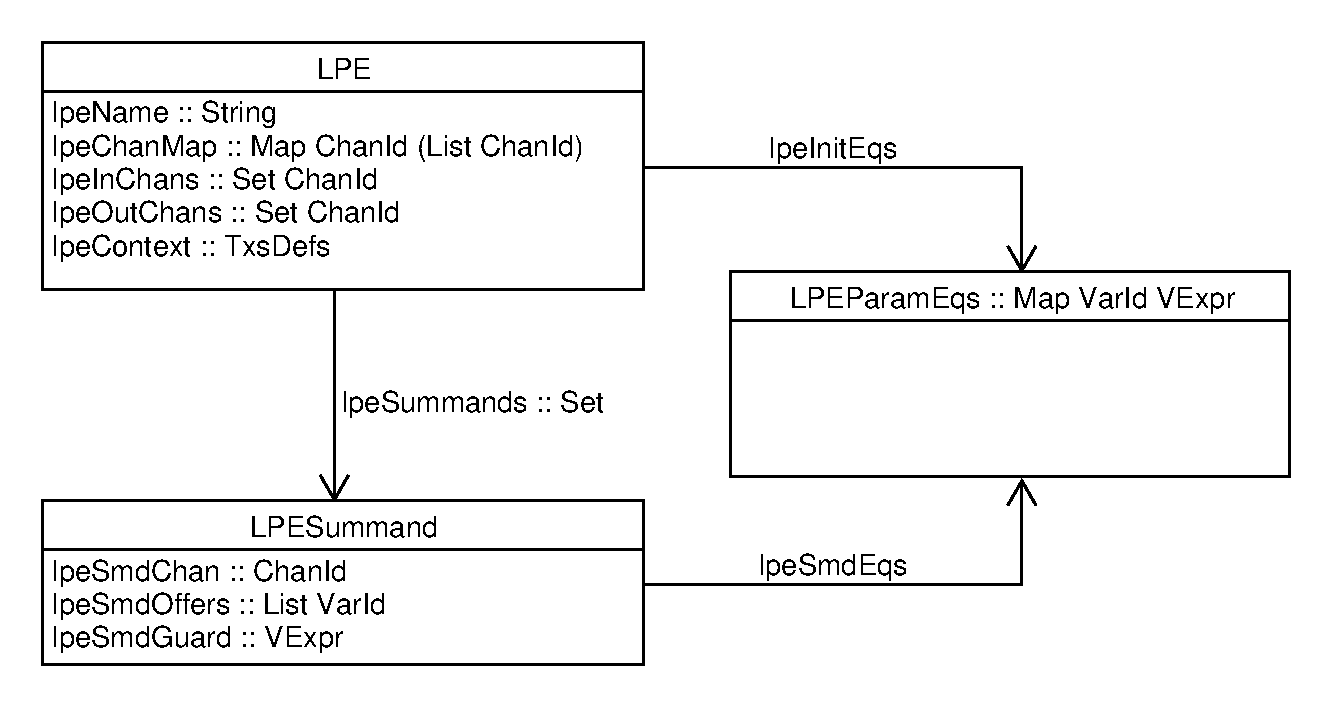
\includegraphics[width=0.7\linewidth]{images/lpe-types}
\caption{LPE data structure.}
\label{lpedatastructure:fig}
\end{center}
\end{figure}

The main data type is \texttt{LPE}.
This type primarily contains information about the \txs{} process in restricted LPE form (see \ref{restrictedlpeform}):
\begin{itemize}
\item The name of the LPE process is \texttt{lpeName};
\item The summands that form the body of the LPE process; and
\item The sorts of the data parameters of the LPE process are contained in \texttt{lpeInitEqs} as well as how each data parameter is initialized.
\end{itemize}

Because the LPE process is always instantiated with the same channels in the same order, the \texttt{LPE} type only has to track which channels are input channels (\texttt{lpeInChans}) and which channels are output channels (\texttt{lpeOutChans}).
Note that these are single channel identifiers that (may) have been freshly generated from multi-channel summands or from summands with hidden variables in order to obtain restricted LPE form (see \ref{restrictedlpeform}).
The \texttt{lpeChanMap} defines how channels in the LPE data structure are converted back to the original channels (it is therefore the implementation of $\Omega_I$ and $\Omega_O$).

The \texttt{LPE} type also stores some circumstantial information in \texttt{lpeContext}.
This is a library of \txs{} type and function definitions that has been copied directly from the original \txs{} model specification.
It is used to validate instances of the \texttt{LPE} type, to generate default values of a specific sort, and more.

Finally, the \texttt{LPESummand} type only contains information about a specific summand: \texttt{lpeSmdChan} is the channel over which it communicates; \texttt{lpeSmdOffers} are the communication variables (including variables that originally were hidden variables); and the \texttt{lpeSmdEqs} map defines which expressions are used to assign new values to the parameters of the LPE after the application of the summand.

\section{Summand elements} \label{summandelements}

To formally reference the elements of $s_i$ -- the $i$th summand of restricted LPE $P$ (see \ref{restrictedlpeform}) -- the following definition is used:
\begin{align*}
s_i = C_i \; \texttt{?} \; x_i(1) \; \cdots{} \; \texttt{?} \; x_i(m_i) \; [[g_i]] \text{ \texttt{>->} } P(v_i(p_1), \cdots{}, v_i(p_k))
\end{align*}

where

\begin{itemize}
\item $C_i$ is the name of the channel over which summand $s_i$ communicates;
\item $m_i \geq 0$ is the number of variables that summand $s_i$ uses to communicate over channel $C_i$;
\item $x_i(j)$ is the $j$th variable that summand $s_i$ uses locally (communication variables first, followed by hidden variables);
\item $g_i$ is the guard of summand $s_i$ (the only free variables in this expression must be parameters of $P$, communication variables of summand $s_i$, or hidden variables of summand $s_i$);
\item $p_1, \cdots{}, p_k$ are the parameters of $P$, of which there are $k \geq 0$;
\item $v_i(p)$ is an expression that defines the new value of parameter $p$ of $P$ after the application of summand $s_i$ (the only free variables in this expression must be LPE parameters, communication variables of summand $s_i$, or hidden variables of summand $s_i$).
\end{itemize}

Note that, because $P$ is in restricted LPE form, the following assumption generally holds for two summands, $s_\alpha$ and $s_\beta$:
\begin{align*}
C_\alpha = C_\beta \rightarrow m_\alpha = m_\beta
\end{align*}

